\documentclass[smallextended]{svjour3}

\usepackage{booktabs} % For formal tables

\usepackage{amsmath}
\usepackage{tikz}
\usepackage{pgfplots}
\pgfplotsset{compat=1.3}
\usepackage{graphicx, epsfig}
\usepackage{xspace}  %% Package used for the \NB{} abbreviation
\usepackage{algorithm}
\usepackage{algpseudocode}
\usepackage{color}
\usepackage{url}
\usepackage{hyperref}
\usepackage{listings}
\usepackage{tikz}% http://ctan.org/pkg/pgf
\usetikzlibrary{calc}
\usepackage{amssymb,amsmath}
\usepackage{subcaption}
%\lstset{
%  basicstyle=\small\ttfamily,
%  columns=fullflexible,
%}

\lstset{language=C++,
 basicstyle=\ttfamily\lst@ifdisplaystyle\scriptsize\fi,%\scriptsize, %aboveskip={-5ex},
 columns=fullflexible,
%basicstyle={\ttfamily\singlespacing},aboveskip={-4ex},
 keywordstyle=\color{blue}\ttfamily,
 stringstyle=\color{red}\ttfamily,
 commentstyle=\color{cyan}\ttfamily,
 captionpos=t,
  %numbers=none, %left,
 numbers=left,
  %numberstyle=\scriptsize,
  %stepnumber=1,
  %numbersep=6pt,
  showstringspaces=false,
  breaklines=true,
  frame=lines,
  otherkeywords={[[,]],::,constexpr},
  emph={rpr,kernel,target,in,out,pipeline,stream,farm,pipe,map,sync,async, rprmv, base, split, unroll, Pipeline, Farm, parallel_execution_ff},
  emphstyle={\color{magenta}\bfseries}
}


% Copyright
%\setcopyright{none}
%\setcopyright{acmcopyright}
%\setcopyright{acmlicensed}
%\setcopyright{rightsretained}
%\setcopyright{usgov}
%\setcopyright{usgovmixed}
%\setcopyright{cagov}
%\setcopyright{cagovmixed}


% DOI
%\acmDOI{10.475/123_4}

% ISBN
%\acmISBN{123-4567-24-567/08/06}

%\acmArticle{4}
%\acmPrice{15.00}

% These commands are optional
%\acmBooktitle{Transactions of the ACM Woodstock conference}
%\editor{Jennifer B. Sartor}
%\editor{Theo D'Hondt}
%\editor{Wolfgang De Meuter}


\begin{document}
\title{Restoration of Legacy Parallelism in C and C++ Applications}
%
%\titlerunning{Abbreviated paper title}
% If the paper title is too long for the running head, you can set
% an abbreviated paper title here
%
\author{Vladimir Janjic         \and
	Christopher Brown \and 
	Adam D. Barwell \and
}

%\authorrunning{Short form of author list} % if too long for running head

\institute{
		V. Janjic \at
	School of Science and Engineering, University of Dundee, UK. \\
	\email{vjanjic001@dundee.ac.uk}
	\and
	C. Brown, A. Barwell \at
	School of Computer Science, University of St Andrews, UK. \\
	\email{cmb21,adb23@st-andrews.ac.uk}           %  \\
}

\date{Received: date / Accepted: date}
% The correct dates will be entered by the editor

\maketitle
%
\begin{abstract}
    \emph{Parallel patterns} are a high-level programming paradigm that enables non-experts in parallelism to develop structured parallel programs that are maintainable, adaptive and portable whilst also achieving good performance on a variety of parallel systems. However, there still exists a large base of \emph{legacy-parallel code} that was developed using ad-hoc methods and incorporating low-level parallel/concurrency libraries such as \emph{pthreads} without any parallel patterns in the fundamental design. This code would benefit from being restructured and rewritten into pattern-based code. However, the process of rewriting the code is tedious and error-prone, due to typical concurrency and pthreading code being closely intertwined throughout the business logic of the program. In this paper, we present a new software restoration methodology, to transform legacy-parallel programs implemented using e.g. \emph{pthreads} into their structured patterned equivalent. We demonstrate our restoration technique on a number of benchmarks, allowing us to introduce patterned parallelism in the resulting code; we record improvements in cyclomatic complexity and speedups.

\keywords{Parallel patterns, restoration, pthreads, refactoring, code analysis}
\end{abstract}

%
% The code below should be generated by the tool at
% http://dl.acm.org/ccs.cfm
% Please copy and paste the code instead of the example below.
%

%\section{To-Do List}
%
%\begin{itemize}
%\item General: Rewrite the paper to focus less on methodology and more on transformations and refactoring
%\item Add a section about dynamic trace-based pattern discovery that we do
%\item Shorten out the Software Restoration section
%\item Have two section on refactoring:
%  \begin{itemize}
%  \item One with ``lower-level'' refactorings, eliminating \lstinline{pthread_create}, locks etc.
%    \item One with ``high-level'' refactorings to eliminate patterns
%    \end{itemize}
%  \item Look at the PARSEC benchmark suite and see what applications we can refactor
%  \item Look at the SE metrics and decide which ones to use in evaluation
%    \item Evaluate the technique with chosen metrics and chosen use cases
% \end{itemize}

\section{Introduction}

Parallel patterns are a well established high-level parallel programming models for producing portable, maintainable, adaptive and efficient parallel code. They have been endorsed by some of the biggest IT companies, such as Intel and Microsoft, who have developed their own parallel pattern libraries (Intel TBB, Microsoft PPL etc.) A standard way to use these libraries is to start with the sequential code base, identifying in it the portions of code that are amenable to parallelisation together with the exact parallel pattern to be applied and then instantiating the identified pattern at the identified location in the code, after possibly restructuring the code to accommodate for parallelism. 

%Figure~\ref{fig:matmult} shows an example of sequential and parallel patterned-code of Matrix Multiplication, one of the most common parallel benchmarks. 

%\begin{small}
%  \begin{lstlisting}[caption=Pthreads Matrix Multiplication\label{lst:matmult_seq}]
%double multiply_row_by_column (double **mat1, int row, double **mat2, int col)
%{
%  int k;
%  double sum=0;
%  for (k=0; k<dim; k++)
%    sum += mat1[row][k] * mat2[k][col];%

%  return sum;
%}

%void multiply_row_by_matrix (double **mat1, int row, double **mat2, double **res)
%{
%  for (int col=0; col<dim; col++)
%    res[row][col] = multiply_row_by_column (mat1, row, mat2, col);

%}

%static void * thread_func (void* arg)
%{
 % input_data *input = (input_data *)arg;
 % for (unsigned int i = input->row_start; i < input->row_end; i++) {
 %         multiply_row_by_matrix(a, i, b, res);
 % }

%  return (void *)0;
%}

%void matrix_muliply()
%{
%  pthread_attr_t attr;
%  int status;%

%  in = (input_data *) malloc (sizeof(input_data) * thread_count);
%  threads = (pthread_t *) malloc (sizeof(pthread_t) * thread_count);
  
%  status = pthread_attr_init(&attr);
%  if (status != 0)
%    std::cout << "Init attributes object" << std::endl;

%  int chunk_size = dim / thread_count;
%  int count = 0;

%  for (unsigned int thread_ind = 0; thread_ind < thread_count; thread_ind++) {
%    /* Setting some generic parameters for each thread */
%    in[thread_ind].row_start = count;
 %   in[thread_ind].row_end = count + chunk;
  %  count += chunk;

   % status = pthread_create(&threads[thread_ind], &attr, &thread_func, &in[thread_ind]);
%    if (status != 0)
 %     handle_error("Creating thread failed!");

 % }%
%}
 % \end{lstlisting}
  
%\end{small}

Sequential code gives the cleanest starting point for introduction of parallel patterns. There exists, however, a large base of \emph{legacy} code  that was parallelised using lower-level, mostly ad-hoc parallelisation methods and libraries, such as \emph{pthreads}~\cite{10.5555/263953}. This code is usually very hard to read and understand, is tailored to a specific parallelisation and optimised for a specific architecture, effectively preventing alternative (and possibly better) parallelisations and limiting portability and adaptivity of the code. An even bigger problem, from the software engineering perspective, is the maintainability of the legacy-parallel code: commonly, the programmer who wrote it is the only one who can understand and maintain the code. This is due to both complexity of low-level threading libraries and the need for custom-built data structures, synchronisation mechanisms and sometimes even thread/task scheduling implemented in the code. 
  
In this paper, we present a new technique for semi-automatic refactoring of the legacy-parallel code into an equivalent sequential form. This makes it significantly easier to introduce structured parallelism that will be equivalent to the ad-hoc parallelism of the original code. This is also the first step towards our \emph{software restoration} methodology, the ultimate goal of which is to provide semi-automatic way of converting legacy-parallel code in to an equivalent patterned code, therefore increasing its maintainability, adaptivity and portability while keeping the similar or, in some cases, even improving the performance. 

This paper makes the following specific research contributions:
\begin{enumerate}
    \item We present a novel software restoration technique for converting legacy-parallel applications into their structured parallel equivalents;
    \item We present a new set of \emph{restoration} refactorings that i) eliminate \lstinline{pthreads} code from legacy C programs, ii) perform \emph{code repair} by further refactoring the code so that it eliminates and bugs introduced by the parallelism elimination stage, and iii) \emph{shaping} refactorings, that prepare the code for parallel pattern introduction, using standard techniques;
    eliminate parallelism from the legacy-parallel \lstinline{pthreads} code, providing semi-automatic implementation of the first step of software restoration methodology;
    \item We evaluate these refactorings on a set of benchmarks, demonstrating that removal of parallelism can allow us to manually derive the structured parallel code that is comparable to the original legacy-parallel version in terms of performance, while being more portable, adaptive and maintainable.
\end{enumerate}

\section{Background} \label{sec:background}
\textcolor{red}{cb: nice section. I think would improve would be to bullet list the exact disadvanages to legacy parallelism and also advantages to using patterns instead?}
Legacy-parallel code, written in ad-hoc way using low level parallel libraries such as \emph{pthreads}, is still very much present in various software repositories and projects. This code was usually developed by parallelism experts before the libraries and programming models for structured parallelisation became popular. It is usually tailored to one specific target machine and architecture, and might use highly-customised parallelisation and associated data structures. This makes it very hard to maintain that code, an increasing important feature in software engineering, or to port it to new architectures. It would be ideal if we could transform every legacy-parallel application into a structured parallel programs, written using high-level parallel programming libraries. However, for this to be possible, it is necessary that a well-defined underlying pattern of parallelism actually exists in the code, which can be exploited by instances of patterns. This is not always the case. However, in substantial number of cases, the parallelism in the application is an instance of one of the common patterns, such as farm, pipeline, workpool or stencil. In these cases, it should be possible, automatically or semi-automatically, to \emph{replace} unstructured parallelism with its structured (patterned) equivalent.   

\subsection{Parallel Patterns}
%\begin{itemize}
%\item What are parallel patterns
%\item Some common patterns
%  \item Benefits of using patterns
%  \item Relevant pattern libraries (Open MP, Intel TBB...)
%\end{itemize}

\noindent
\emph{Parallel patterns} are a high-level abstraction for representing classes of computations that are similar in terms of their parallel structure, but different in terms of problem-specific operations. A typical example of a parallel pattern is a \emph{parallel map}, where the same operation is applied to a set of independent inputs in parallel. 
%Regardless of whether the actual operation is, for example, multiplying a matrix by a vector, processing a pixel of an image or XX, the parallel structure of the computation will be the same. Parallel Patterns are typically implemented as library functions which handle creation, synchronisation and communication between the parallel threads, while the problem-specific (often sequential) computations are provided as the pattern parameters. 
In this paper, we restrict ourselves to two classical parallel patterns, which we believe to be the most common. Note that the technique described in this paper can be further generalised to include the full tractable set of parallel patterns.
\begin{itemize}
    \item The farm pattern models a data parallel computation, where a single computational worker, $f$, is applied to a set of independent inputs, $x_{1}, ..., x_{n}$. The parallelism arises from applying the worker, $f$, to different input elements at the same time in parallel. 
    \item The pipeline pattern models a parallel pipeline. Here, a sequence of functions, $f_{1}, f_{2}, ..., f_{m}$ are applied to a stream on independent inputs, $x_{1}, ..., x_{n}$. The output of $f_{i}$ becomes the input to $f_{i+1}$, so that the parallelism arises from executing $f_{i+1}(f_{i}(...f_{1}(x_{k})...))$ in parallel with $f_{i}(f_{i-1}(...f_{1}(x_{k+1})...))$.
\end{itemize}

The benefits of using parallel patterns lie in clear separation between sequential and parallel parts of the code and high-level description of the underlying parallelism, which makes the patterned applications much easier to maintain, change and adapt to new architectures. 
%For these reasons, they have been endorsed by most of the top IT companies, who have their own pattern libraries, such as Microsoft PPL~\cite{ppl} and Intel Thread Building Blocks~\cite{tbb}. In addition to that, there are also many popular open-source pattern libraries, such as OpenMP~\cite{openmp} and FastFlow~\cite{openmp}.

\subsection{Reading and Writing} \label{sec:readwrite}
In Section~\ref{sec:refactoring}, we make use of matching various instances of \emph{read} and \emph{write} operations in the source-code. We use standard language definitions for reading and writing to variables.
If a variable \lstinline{x} appears on the left-hand-side of an assignment, we class the operation as a \emph{write} (here, the variable, \lstinline{x} is assigned the value of the expression, \lstinline{e}).

\begin{lstlisting}
x = e;
\end{lstlisting}

\noindent
If a variable appears in an expression, or on the right-hand-side of an assignment, we class the operation as a \emph{read}. Here, the contents of variable \lstinline{y} are \emph{read}, and \emph{written} to variable \lstinline{x}.

\begin{lstlisting}
x = y;
\end{lstlisting}

\subsection{Software Refactoring}
\noindent
\emph{Software refactoring} is the process of changing the structure of a program while preserving
its functional semantics in order, for example, to increase code quality, programming
productivity and code reuse. In our case, refactorings are source-to-source transformations of the code that are performed \emph{semi-automatically}, under the programmers guidance and possibly with his input. In our previous work, we pioneered refactoring to introduce parallelism~\cite{rpl}, where sequential code is transformed to introduce instances of parallel patterns. We have shown that this can lead to excellent speedups of the resulting code. Although the term refactoring was first introduced by Opdyke in his PhD thesis in 1992~\cite{opdyke}, and the concept goes at least as far back as the fold/unfold system proposed by Burstall and Darlington in 1977~\cite{darlington77}. In our case, refactorings are source-to-source transformations of the code that are performed \emph{semi-automatically}, under the programmer's guidance, and possibly with their input. 
ParaFormance \footnote{\url{http://www.paraformance.com}} is a refactoring tool-suite developed at the University of St Andrews that refactors C and C++ programs into parallel versions. It targets a number of different back-ends, including FastFlow, Intel Thread Building Blocks (TBB), OpenMP and GrPPI. It has a number of unique features and is integrated as a plugin into both Eclipse and Microsoft Visual Studio, presenting a menu of various options to its users.

% ParaFormance provides \emph{semi-automated refactorings} to introduce parallel patterns into sequential code; \emph{safety checking} features to find, statically, parallelism related bugs, such as race-conditions, deadlocks and memory collisions; and \emph{pattern discovery}, to find the hotspots in the program that are suitable for parallelism. All refactorings applied to source code in ParaFormance are fully undoable. Furthermore, all operations in ParaFormance come with a full preview feature, enabling users to see the result of the transformation before applying it. 
%Figure~\ref{fig:safety1} gives a screenshot of the ParaFormance tool integrated into Eclipse. 




\section{Software Restoration}
%\textcolor{red}{cb: not sure we need the subseciton in the background if we have this section, or we can maybe omit or drastically cut this section down}

\noindent
\emph{Software restoration} is a methodology %based on software refactoring and code analysis
for improving structure of the legacy-parallel C++ code by applying a series of incremental program analysis and transformation steps to rewrite the code into its patterned equivalent. %In this way, w
Software restoration is based on software refactoring and code analysis and aims to:
\begin{itemize}
\item \emph{discover} the instances of common patterns in legacy-parallel code;
\item \emph{eliminate} the \emph{undesirable} parallelism from the same code;
\item \emph{replace} the removed parallelism with instances of the parallel patterns;
\end{itemize}
\noindent
The input to the Software Restoration process is a legacy-parallel C/C++ code that is based on some low-level parallelism library, such as pthreads, and the output is the semantically-equivalent code based on parallel patterns. In this way, we obtained well-structured code based on higher level of parallel abstraction, which is significantly more maintainable and adaptive while still preserving
good performance of the original, highly-tuned parallel version. In this paper, we will focus on the GrPPI library as our target code. This allows us to then generate the final code for a number of different parallel backends, such as Intel TBB, OpenMP and Fastflow.

Software Restoration methodology consists of a number of steps, each applying a class of code transformations, some of which are driven by the pattern discovery code analysis.  The whole process is depicted in Figure~\ref{fig:SoftRest}. In the description below, we will focus on the code transformation steps. As a running example to demonstrate the transformation, we will use a synthetic parallel pipeline code, given in the Listing~\ref{lst:simplePipe}.


\begin{figure*}
\centering
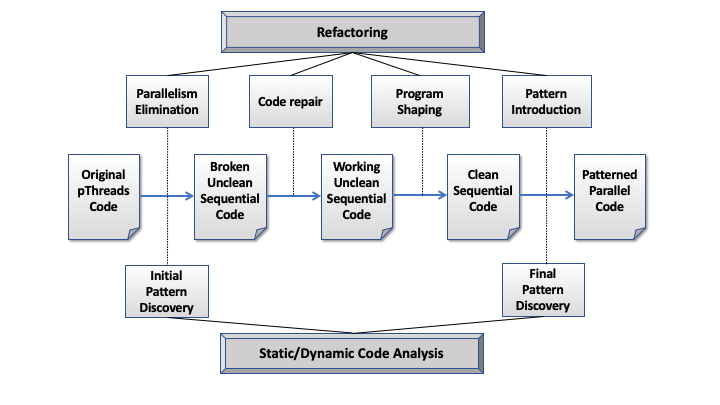
\includegraphics[width=\textwidth]{images/HLPP2020Paper.png}
\caption{Software Restoration Process}
\label{fig:SoftRest}
\end{figure*}

%\begin{figure}
\begin{lstlisting}[caption=Original Simple Pipeline Code,frame=single,label=lst:simplePipe]
  int main(int argc, char *argv[]) {
  ...  
    /* create the workers, then wait for them to finish */
    pthread_create(&workerid[0], &attr, Stage1, (void *)&stage_queues[0]);
    pthread_create(&workerid[1], &attr, Stage2, (void *)&stage_queues[1]);
    pthread_create(&workerid[2], &attr, Stage3, (void *)&stage_queues[2]);
    
    for (i = 0; i < NRSTAGES; i++)
    pthread_join(workerid[i], NULL);
    
    ...
  }

  /* Second stage reads an element from the input queue, adds 1 to it and writes it to the output queue */
  void *Stage2(void *arg) {
    int my_input;
    int my_output;
    
    pipeline_stage_queues_t *myQueues = (pipeline_stage_queues_t *)arg;
    queue_t *myOutputQueue = myQueues->outputQueue;
    queue_t *myInputQueue = myQueues->inputQueue;
    
    do {
      my_input = read_from_queue(myInputQueue);
      if (my_input > 0)
      my_output = my_input + 1;
      else /* 0 is a terminating token...If we get it, we just pass it on... */
      my_output = 0;
      add_to_queue(myOutputQueue, my_output);
    } while (my_input>0);
    
    return NULL;
  }

  void add_to_queue(queue_t *queue, int elem)
  {
    pthread_mutex_lock(&queue->queue_lock);
    /* If the queue is full, wait until something reads from it before adding a new element */
    if (queue->nr_elements == queue->capacity) {
      pthread_cond_wait(&queue->queue_cond_read,&queue->queue_lock);
    }
    queue->elements[queue->addTo] = elem;
    queue->addTo = (queue->addTo + 1) % queue->capacity;
    queue->nr_elements++;
    pthread_cond_signal(&queue->queue_cond_write);
    pthread_mutex_unlock(&queue->queue_lock);
  }

\end{lstlisting}

\noindent
The above listing shows a snipet of the code. In the main function (lines 1--12), a pipeline of three stages is created using three threads. The stages are connected by queues, so that each stage (apart from the first one) has its input and output queue. After the thread creation, the main function just waits for the threads to finish their work (lines 8--9). In the lines 15--33, we show the function for the middle stage of the pipeline. This function simply reads an element from the input queue (an integer number), adds 1 to it and then puts it into the output queue. All the synchronisation code is in the \lstinline{add_to_queue} and \lstinline{remove_from_queue} functions. We show just the \lstinline{add_to_queue} function (lines 35--47), as \lstinline{remove_from_queue} is quite similar. That function uses one lock and two conditional variables for the queue. The conditional variables are used for synchronisation when threads are waiting for reading from an empty queue (at the start of the program) or for writing into a full queue. When a thread needs to add to the queue, it first grabs the queue lock, then checks if the queue capacity is reached, in which case writing a new element is impossible. In this case, the thread releases a lock and waits for a signal that some other thread has consumed an element of this queue (\lstinline{queue->queue_cond_read} conditional variable at line 40). After this conditional variable is signalled, there is space to write a new element into the queue, so the thread writes it and updates the queue counter (lines 42--44). Finally, the thread signals that a write into the queue has occured (\lstinline{queue->queue_cond_write} conditional variable in line 45) and releases the queue lock (line 46) before returning.

\paragraph{Parallelism Removal.}
The initial code analysis step (\emph{Initial Pattern Discovery}) analyses the original pthreads code and discovers part of it that correspond to instances of parallel patterns. In our example, this stage identifies the pipeline created in lines 4--6, with the pipeline stages being functions \lstinline{Stage1}, \lstinline{Stage2} and \lstinline{Stage3}. After that, the first code transformation step is applied, where we remove the threaded code replace it with the sequential equivalent. This includes the calls to \emph{pthreads} functions for thread creation, synchronisation, mutex management and so on. In our example, this would impact the \lstinline{main} and \lstinline{add_to_queue} functions, which would become as in the Listing~\ref{lst:pipeParRem}.

\begin{lstlisting}[caption=Simple Pipeline Code with Parallelism Removed, frame=single, label=lst:pipeParRem]
  int main(int argc, char *argv[]) {
  ...  
    /* create the workers, then wait for them to finish */
    Stage1((void *)&stage_queues[0]);
    Stage2((void *)&stage_queues[1]);
    Stage3((void *)&stage_queues[2]);

    /* pthread_join would be removed
    for (i = 0; i < NRSTAGES; i++)
      pthread_join(workerid[i], NULL);
    */
      
    ...
  }

   void add_to_queue(queue_t *queue, int elem)
  {
    /* All of the locks and conditional variables would be removed */

    queue->elements[queue->addTo] = elem;
    queue->addTo = (queue->addTo + 1) % queue->capacity;
    queue->nr_elements++;

  }
\end{lstlisting}

\noindent
Note that all the \lstinline{pthread_} calls from the Listing~\ref{lst:simplePipe} have either been removed or replaced with the calls to the underlying functions (in the case of \lstinline{pthread_create}). Note, however that the code obtained in this
way would not work. In particular, \lstinline{Stage1} function would be executed, which would just write all its outputs into its output queue (in a circular way), therefore overwriting the data possibly multiple times. After \lstinline{Stage1} finishes,
\lstinline{Stage2} would start, read all the elements currently in its input queue (which would be just a subset of all the data produced by \lstinline{Stage1}) and write them to the output queue. It is clear that in this way there would be loss of data, so the output that the final stage produces would not be the same as in the parallel version.

\paragraph{Code Repair.}
As we observed in the previous step, the parallelism removal step might result in a code that is broken and, hence, is not semantically equivalent to the original legacy-parallel code. Our example is just one of many instances in which merely removing the \lstinline{pthread} constructs actually breaks the code. The next step in Software Restoration is, therefore, to repair the potentially broken code that is the output of the previous step. In our pipeline example, this is actually the most complicated step of the whole methodology and the resulting code is given in Listing~\ref{lst:pipeRepaired}.

\begin{lstlisting}[caption=Simple Pipeline Code after Code Repair, frame=single, label=lst:pipeRepaired]

  int main(int argc, char *argv[]) {
  ...  

    while (output_stage_1>0) {
      output_stage_1 = Stage1((void *)&stage_queues[0]);
      Stage2((void *)&stage_queues[1]);
      Stage3((void *)&stage_queues[2]);
    }
      
  ...
  }

  /* Second stage reads an element from the input queue, adds 1 to it and writes it to the output queue */
  void *Stage2(void *arg) {
    int my_input;
    int my_output;
    
    pipeline_stage_queues_t *myQueues = (pipeline_stage_queues_t *)arg;
    queue_t *myOutputQueue = myQueues->outputQueue;
    queue_t *myInputQueue = myQueues->inputQueue;
    
    my_input = read_from_queue(myInputQueue);
    if (my_input > 0)
    my_output = my_input + 1;
    else /* 0 is a terminating token...If we get it, we just pass it on... */
    my_output = 0;
    add_to_queue(myOutputQueue, my_output);
    
    return my_input;
  }
\end{lstlisting}

\noindent 
In the listing, we show the \lstinline{main} and \lstinline{Stage2} function. Note that in the main function, the three stages of the pipeline are interleaved in the while loop (lines 4--9). The \lstinline{Stage2} function is transformed so that it performs just one iteration, with the loop in the function being eliminated. The terminating condition has been lifted from the
\lstinline{Stage1} function into the newly introduced loop at line 4. Therefore, in the newly introduced loop, \lstinline{Stage1} generates one element and puts it into its output queue, \lstinline{Stage2} consumes the element from this output queue, processes it and puts its output in its own output queue and then \lstinline{Stage3} consumes the element from this queue, processes it and puts its output into the final queue. This is repeated until \lstinline{Stage1} generates the terminating element (\lstinline{0} in this case).

\paragraph{Program Shaping.}
After the code repair step, the resulting code will be working sequential C/C++ code that can be compiled, and which can be transformed into the patterned parallel version. However, some artefacts of the legacy parallelisation may still remain in the code. In our example, these are the queues between stages of the pipeline computation, but in other examples it can also be custom-build representations of flat data structures, such as arrays. These artefacts are redundant and might actually hinder alternative (and possibly better) parallelisations of the code. The next step is, therefore, to eliminate them and restore the code in as clean state as it is possible. For our example, the resulting code (\lstinline{main} and \lstinline{Stage2} functions) are given in Listing~\ref{lst:pipeClean}.

\begin{lstlisting}[caption=Clean Sequential Simple Pipeline Code, frame=single, label=lst:pipeClean]

  int main(int argc, char *argv[]) {
  ...  

    while (output_stage_1>0) {
      int output_stage_1 = Stage1();
      int output_stage_2=Stage2(output_stage_1);
      int output_stage_3=Stage3(output_stage_3);
      printf(``%d\n'', output_stage_3
    }
      
  ...
  }

  /* Second stage reads an element from the input queue, adds 1 to it and writes it to the output queue */
  int Stage2(int input) {
    int my_output;
    
    if (input>0)
      my_output = input + 1;
    else /* 0 is a terminating token...If we get it, we just pass it on... */
      my_output = input;
    
    return my_output;
  }
\end{lstlisting}

%\item \emph{Feature Cleanup.}  After the application of parallelism removal transformations, some artifacts of the legacy parallelisation may still remain in the code. These can be, for example, queues between stages of the pipeline computation or custom-build representations of flat data structures, such as arrays. These artifacts do not prevent the sequential version of application from running, but are redundant and might actually hinder alternative (and possibly better) parallelisations of the code. The next step is, therefore, to eliminate these artifacts and restore the code in the state as close to the original sequential code from which legacy parallelisation was derived as is possible. This is, again, done using refactorings. As we are focusing on the \emph{farm} and \emph{pipeline} parallelism, the transformations we do is removing the queues of the pipeline stages (for the \emph{pipeline} parallelism) and flattening of data structures (in the case of \emph{farm} parallelism). The Matrix Multiplication code after feature cleanup is given below

%% \begin{lstlisting}
%% static void *func (void* arg)
%% {
%%   data *input = (data *)arg;
%%   for (int i = input->start; i < input->end; i++) {
%% 	  multiply_row_by_matrix(a, i, b, res);
%%   }
%%   return (void *)0;
%% }


%% void threads_create() {
%%   int status;
%%   int count=0;
%%   in = (data *) malloc (sizeof(data) * tc);

%%   #pragma farm(func,tc)   
%%   for (int tid=0; tid<tc; tid++) {  
%%     in[tid].start = count;
%%     in[thread_ind].row_end = count + chunk;
%%     count += chunk;

%%     func(&in[tid]);
%%   }
%% }
%% \end{lstlisting}
%% The array \lstinline{in} in the Matrix Multiplication code represented a block view of the flat array of indices of the matrix rows, which was introduced for the purpose of chunking to increase parallelism granularity in the legacy parallelisation based on the \emph{farm} parallelism. The array of all the rows of matrix \lstinline{b} was divided in as many chuncks as there are threads (\lstinline{tc}) and a chunk of this array assigned to each thread. Since modern pattern libraries, such as \emph{OpenMP} and \emph{TBB} can do chunking implicitly and dynamically, based on e.g.~the current system load, there is no need for explicit chunking to remain in the sequential code, even if it is going to be turned into patterned code again. Therefore, we eliminate the array \lstinline{in} and change the loop on line XX to iterate over the array of matrix rows instead.  
  
%\item \emph{Additional Pattern Discovery.} Finally, once the code is restored into the state that is as close to the original sequential version as possible, further pattern discovery analysis can be made on it, as the feature cleanup transformations, and especially flattening of data structures and elimination of intermediate buffers/queues, might result in the code that has additional instances of parallel patterns that were not detected on the original, legacy-parallel code. This might enable us to parallelise the code in a different way than it was done in the original, legacy-parallel version, bringing possible benefits even in terms of performance.


\paragraph{Pattern Introduction.}
After the final pattern discovery analysis is performed and the final patterns to be introduced are identified, together with the locations in the code where this will be done, the final step is to introduce instances of parallel patterns into the now-clean sequential code. The parts of the sequential code are replaced by calls to the functions from the high-level pattern libraries such as \emph{Intel TBB}~\cite{DBLP:reference/parallel/X11pz} or \emph{OpenMP}~\cite{10.1109/99.660313}. This results in final, patterned parallel code that is semantically equivalent to the starting legacy-parallel code, but with much cleaner structure and simpler, higher-level code that allows easier maintainability, adaptivity and portability.
%\end{itemize}

\section{Restoration Refactorings} \label{sec:refactoring}

In this section we propose three refactorings to \emph{restore} C applications that have been previously parallelised using low-level pthread parallelism techniques. We divide our restoration refactorings into specific examples of eliminating \emph{pipeline} parallel (described in Section~\ref{sec:removepipeline}), and removing \emph{farm} parallelism (described in Section~\ref{sec:removefarm}).
These restoration refactorings on both farm and pipelines are categorised by i) \emph{eliminating} the existing pthread concurrency by removing the calls to pthread functions, to they can be later replaced with calls to structured high-level algorithmic skeletons (described in Section~\ref{sec:removepthread}), ii) \emph{repairing} the eliminated versions of the code, which may have some bugs introduced by removing the underlying concurrency logic, and iii) \emph{shaping} the code, into order to structure it in a way that parallel patterns can be easily introduced. 
We explain each of these refactorings one by one in the following subsections.

\subsection{Removing Pthread Concurrency} \label{sec:removepthread}



\begin{enumerate}

\item \textbf{Replace \lstinline|pthread_create| with a function call}

This refactoring replaces a call to \lstinline|pthread_create| with a function call. Any formal arguments that were originally passed to the thread, are passed to the function instead. The return result of the function, originally captured as a variable argument to \lstinline|pthread_create| is assigned to the variable instead. For instance, the example 


	\begin{lstlisting}[frame=single]
	var = pthread_create(&thread, NULL, f, args);
	\end{lstlisting}

can be refactored into:


	\begin{lstlisting}[frame=single]
	var = 0;
	f(args);
	\end{lstlisting}


Here \texttt{var} is assigned \texttt{0} in lieu of the original return value of \lstinline|pthread_create| when the call is successful. The refactoring assumes that \lstinline|f| 
%communicates with other threads via mutexes or semaphores, and 
does not itself return a non-null value \emph{via} \lstinline|pthread_exit|. The refactoring can therefore only be applied when the body of \lstinline|f| contains only calls to \lstinline|pthread_exit| to which \lstinline|NULL| is passed as its argument. % \forall pthread_exit(var) \in f.statements.transclosure, var = NULL
If the \lstinline{pthread_create} is within some arbitrary nesting of statements or expressions, then the same refactoring can still be applied, by first lifting (and therefore introducing an assignment of) the \lstinline{pthread_create} call first, therefore arriving at the refactored example above.

\item \textbf{Replace \lstinline|pthread_exit| with a return statement}

This refactoring replaces a call to \lstinline|pthread_exit| with a return statement. The argument originally passed to \lstinline|pthread_exit| are instead passed to the return statement. Consider the following example.

\begin{lstlisting}[frame=single]
pthread_exit(var);
\end{lstlisting}

\noindent
is refactored into

\begin{lstlisting}[frame=single]
return var;
\end{lstlisting}

\noindent
where \lstinline|var| may either be a variable or \lstinline|NULL|. Unlike the refactorings that replace \lstinline|pthread_create| and \lstinline|pthread_join|, this refactoring does \emph{not} require \lstinline|var| to be \lstinline|NULL| since both cases can be refactored in the same way. Although trivial, this is an important transformation step to removing concurrency that forms our complete methodology.


%Whilst this refactoring allows for spawned functions to return values \emph{via} \lstinline|pthread_exit| and \lstinline|pthread_join|, the other refactorings defined and used herein assume that only functions that 

%\noindent
%\emph{Note that if \lstinline|var| \emph{isn't} \lstinline|NULL| then the result of the refactored \lstinline|pthread_create| needs to be captured. (Where? At the point of \lstinline|pthread_join|? At the point of \lstinline|pthread_create|?) Assume it only returns \lstinline|NULL| for consistency?}

\item \textbf{Remove \lstinline|pthread_join|}

This refactoring removes a call to \lstinline|pthread_join| when its second argument is \lstinline|NULL|; i.e.\ when it does \emph{not} expect a value to be returned from the exiting thread. As with \lstinline|pthread_create|, when the result of a call to \lstinline|pthread_join| is assigned to a variable, e.g.\

\begin{lstlisting}[frame=single]
var = pthread_join(thread, NULL);
\end{lstlisting}

\noindent
the statement is refactored into the assignment:

\begin{lstlisting}[frame=single]
var = 0;
\end{lstlisting}

\noindent
where \lstinline|0| is again the value returned by \lstinline|pthread_join| when it is successful. 

%\emph{Again, what happens when it's part of another statement (e.g.\ if-statement) or another expression? Lift into a variable and replace call sites with that variable. In which cases does the change in order of expressions affect the external behaviour?}

\end{enumerate}

%\subsection{Farm Removal}
%
%\begin{itemize}
%\item Matrix Multiplication example
%  \begin{itemize}
%  \item \texttt{discovery-examples/matmult/matmult\_pthreads.cpp}
%  \end{itemize}
%\item Points of note
%  \begin{itemize}
%  \item Global
%    \begin{itemize}
%    \item \lstinline|#include <pthread.h>|
%    \item \lstinline|pthread_t *threads| (remove assignment in \lstinline|threads_create|)
%    \end{itemize}
%  \item \lstinline|main|
%    \begin{itemize}
%    \item \lstinline|pthread_join(NULL)|
%    \item \lstinline|pthread_exit(NULL)| (transform to: \lstinline|return(NULL)|)
%    \end{itemize}
%  \item \lstinline|threads_create|
%    \begin{itemize}
%    \item \lstinline|pthread_attr_t attr| (remove \lstinline|pthread_attr_init|, replace with \lstinline|status = 0| to satisfy the if-statement at line 105)
%    \item \lstinline|pthread_create| (rewrite to \lstinline|status=0;thread_func(threads[thread_ind])|)
%    \end{itemize}
%  \end{itemize}
%\end{itemize}

\subsection{Pipeline Parallelism Removal} \label{sec:removepipeline}

\begin{lstlisting}[frame=single,numbers=left,label=lst:simplepipeexample,caption={Simple pipeline example, based on PGPry, from the Parsec benchmark suite.}]
..
pthread_t one, two;
int shared = 0;
pthread_mutex_t mut;
void *StageOne(void *threadarg1) {
  for (int i1 = 0; i1 < 5; i1++) {
    pthread_mutex_lock(&mut);
    int loc_shared = shared;      // Read shared
    pthread_mutex_unlock(&mut);
    ...
    pthread_mutex_lock(&mut);
    shared = loc_shared++;     // Update shared
    pthread_mutex_unlock(&mut);
    }
  pthread_exit(NULL);
}
void *StageTwo(void *threadarg2) {
  for (int i2 = 0; i2 < 5; i2++) { 
    pthread_mutex_lock(&mut);
    int loc_shared = shared;     // Read shared
    pthread_mutex_unlock(&mut);
    ...
    pthread_mutex_lock(&mut);
    shared = loc_shared--;      // Update shared
    pthread_mutex_unlock(&mut);
    }
  pthread_exit(NULL);
}
... main () {
  int status;
  status = pthread_create(&one, NULL, StageOne, NULL);   // Stage One
  if (status != 0) exit(-1);
  status = pthread_create(&two, NULL, StageTwo, NULL);  // Stage Two
  if (status != 0) exit(-1);
  pthread_join(one, NULL);
  pthread_join(two, NULL);
}
\end{lstlisting}

%\paragraph]{Very Simple Example.}

%Simplified PGPry example (Listing~\ref{lst:simplepipeexample}). A two-stage pipeline with farms for the stages. An integer represents the (size of a) buffer between stages. Parallelism removal assumes perfect scheduling for the sequential version; practically, we do not see exactly the same behaviour for the sequential version as we do the parallel versions (for all runs of the parallel version).
\noindent
Instances of the \emph{pipeline} pattern (see Section~\ref{sec:background}) occur frequently in legacy code involving pthreads. Typically, these instances incur two or more stages that interact with each other in an implicit way. For example, through the update of a shared variable between threads. For example, Listing~\ref{lst:simplepipeexample} shows a two-stage pipeline example, where each stage is also a \emph{farm}. This example is a simplified version of the PGPry example, taken from the Parsec Benchmark Suite~\cite{10.1145/1454115.1454128}. In the example, an integer is used to represent the size of a buffer between stages (\lstinline|i1| at Line 6, and \lstinline|i2| at Line 18).
These stages are:

\textbf{Stage 1} removes the direct calls to the pthread API, (as described in Section~\ref{sec:removepthread}). For example, this includes in \lstinline|main|, replacing \lstinline|pthread_create| calls with an assignment to \lstinline|status| and a call to the spawned function. This ensures that \lstinline|status| is initialised for the subsequent uses of it; and that values assigned should be the default successful returned value of \lstinline|pthread_create|.
\begin{lstlisting}[frame=single]
// status = pthread_create(&one, NULL, StageOne, NULL);
status = 0;
StageOne(0);
if (status != 0) {
  exit(-1);
}
\end{lstlisting}
\noindent
This stage also considers the \lstinline|pthread_join| calls in \lstinline|main|. Since these do not expect return values (i.e.\ their second argument is \lstinline|NULL|), so they can just be removed.
The final refactoring in this stage is to replace the \lstinline|pthread_exit| calls with \lstinline|return NULL;|

\textbf{Stage 2} unifies the stages of the pipeline together, forming a single unified stage in the form of a newly introduced function, as illustrated in the code below. The free variables in the original stages are captured as arguments to the newly introduced unified stages. Bound variables are declared in the unified stage up to alpha-renaming to preserve freshness and the binding structure of the stages. 

  \begin{lstlisting}[frame=single]
// Stage One:
int i1;
for (i1 = 0; i1 < 5; i1++) {...}
// Stage Two:
int i2;
for (i2 = 0; i2 < 5; i2++) {...}
// Unifies to:
int i1;
int i2;
for (i1 = 0, i2 = 0; i1 < 5 || i2 < 5; i1++, i2++) {...}
\end{lstlisting}
\noindent
Typically, the original stages of the pipeline will contain loops; these will be unified together by forming the disjunction of the conditionals from all the loops.
 This process is done by unifying from the first stage, then the second stage, and so on. There may be duplicated portions of the code as a result of the stage. This duplicate code can be filtered out by using common \emph{clone detection} techniques, commonly found in the literature, such as [BLAH]. Any code that occurs before any \emph{read} or \emph{write} operations on any shared data can simply be inserted into the unified stage. 
 
\begin{lstlisting}[frame=single]
int i1;
int i2;
for (i1 = 0, i2 = 0; i1 < 5 || i2 < 5; i1++, i2++) {
  int loc_shared1 = shared;
  sleep(1); // representing block code
  ...
}
\end{lstlisting}
\noindent
\textbf{Stage 3} attempts to match the \emph{reads} and \emph{writes} to the shared state that occurs in the various original stages of the pipelines. These need to be unified in such a way that order of execution is preserved in the unified stage. Operations on the state can be matched accordingly. Match \emph{read} operations on the shared state with other \emph{read} and \emph{write} operations on the shared state. In the example, a \emph{read} is matched with a \emph{read}, resulting in picking the \emph{read} operation in the first stage; here, the assignment to \lstinline|loc_shared|, occurring in \lstinline|StageOne| and \lstinline|StageTwo| (Lines 8 and 20) of Listing~\ref{lst:simplepipeexample} can be merged together to form a single assignment statement (as illustrated at Line 4 in the listing below).
\begin{lstlisting}[frame=single]
int i1;
int i2;
for (i1 = 0, i2 = 0; i1 < 5 || i2 < 5; i1++, i2++) {
   int loc_shared = shared;
   ...
}
\end{lstlisting}

\noindent
A \emph{write} operation (see Section~\ref{sec:readwrite}) in the first stage is matched with another \emph{write} operation in the second (and subsequent) stages. In Listing~\ref{lst:simplepipeexample}, we see a \emph{write} to the shared variable \lstinline|loc_shared| on Line 12, in \lstinline|StageOne| and also on Line 24, in \lstinline|StageTwo|. Here, we execute the \emph{write} instruction \lstinline|loc_shared++| from \lstinline|StageOne| first, and then we execute the \emph{write} instruction, \lstinline|loc_shared--|, from \lstinline|StageTwo|. Indeed, in this example, there is an interesting observation that these two operations will functionally cancel each other out, as incrementing a variable, and then immediately decrementing it, is obviously a \emph{cancelling} behaviour; however, reasoning about the behaviour of the operations outside of a basic \emph{read/write} behaviour is beyond the scope of this paper.

  \begin{lstlisting}[frame=single]
int i1;
int i2;
for (i1 = 0, i2 = 0; i1 < 5 || i2 < 5; i1++, i2++) {
  int loc_shared1 = shared;
  sleep(1); // representing block code
  shared = loc_shared1++;

  int loc_shared2 = shared;
  sleep(1); // representing block code
  shared = loc_shared2--;
}
\end{lstlisting}

\noindent
\textbf{Stage 4} replaces the original code in the \lstinline{main} function (Lines 29 -- 36 of Listing~\ref{lst:simplepipeexample}) with a call to the new unified function (here renamed to something more meaningful).

  \begin{lstlisting}[frame=single]
int main () {
  int status;
  SynthesisedPipe(NULL, NULL); // StageOne and StageTwo combined.
  if (status != 0) exit(-1);
}
\end{lstlisting}

\noindent
\textbf{Stage 5} the parallelisation of the sequentialised version of the code can now be performed. Here, we now take the introduced function, and derive \emph{pipeline} stages from it, so that a patterned version can be introduced, using a framework like OpenMP~\cite{10.1109/99.660313}, Intel's Threading Building Blocks~\cite{DBLP:reference/parallel/X11pz}, or GrPPI~\cite{DBLP:journals/concurrency/AstorgaD0G17}. Here, any free variables in the refactored functions/pipeline stages need to be captured. Therefore a \lstinline|struct| is declared at Lines 1 and 13, representing the return types of the pipline stages \lstinline|S1| and \lstinline|S2|. Any global variables that previously were assigned to the results of these stages are now captured; for example at Lines 31 and 35. Note here that \lstinline{S2} takes as a parameter the updated variable \lstinline{shared} at Line 33. 

\begin{lstlisting}[frame=single]
int main() {
...
struct pipe_result = SynthesisedPipe(NULL, NULL, shared);
shared = pipe_result.shared;
...
}
\end{lstlisting}
The \lstinline|struct| can be automatically generated itself, where the fields are all free variables (i.e.\ the globals) in the synthesised function.
%
We finally parallelise the refactored code using a clean pattern method of parallelisation, such as GrPPI.

\begin{lstlisting}[frame=single]
void* SynthesisedPipe(void* threadarg1, void* threadarg2, int shared) {
int i1;
int i2;
for (i1 = 0, i2 = 0; i1 < 5 || i2 < 5; i1++, i2++) {
  #pragma grppi seq stage
  tuple1 ret1 = S1(i1, shared);
  i1 = ret1.i1;
  shared = ret1.shared;

  #pragma grppi seq stage
  tuple2 ret2 = S2(i2, shared);
  i2 = ret2.i2;
  shared = ret2.shared;
  }
  return NULL;
}
\end{lstlisting}

%\paragraph{Refactoring stages.}
%\iffalse
%
%
%\begin{enumerate}
%\item In \lstinline|main|, remove farms over pipeline stages by removing the for loops surrounding them.
%\begin{lstlisting}[frame=single]
%for(i = 0; i < NUM_THREADS; i++) {
%  ...
%  rc = pthread_create(&threads[i], NULL, StageOne, arg);
%  ...
%}
%\end{lstlisting}
%Farms are for loops that contain a \lstinline|pthread_create| call. What if the for loops also calculate something else? Assume that a pragma indicating a farm stage is okay for transformation. Alpha renaming of local variables declared inside the loop body where necessary. Result of the above:
%\begin{lstlisting}[frame=single]
%...
%rc1 = pthread_create(&threads[i], NULL, StageOne, arg1);
%...
%\end{lstlisting}
%\item Still in \lstinline|main|, rewrite the \lstinline|pthread_create| calls as function calls.
%\begin{lstlisting}[frame=single]
%rc = 0;
%StageOne(arg1);
%\end{lstlisting}
%As before, since the result of \lstinline|StageOne| is assigned to a \lstinline|status|-type variable, here \lstinline|rc|, we assign the default positive result of \lstinline|pthread_create| to that variable before calling the spawned function, here \lstinline|StageOne|.
%
%\end{enumerate}
%
%\fi
%%
%\begin{enumerate}
%	\item .
%%\item In \lstinline|main|, replace \lstinline|pthread_create| calls with an assignment to \lstinline|status| and a call to the spawned function. Ensures that \lstinline|status| is initialised for the subsequent uses of it; value assigned should be the default successful returned value of \lstinline|pthread_create| (here, that's \lstinline|0|).
%%\begin{lstlisting}[frame=single]
%%// status = pthread_create(&one, NULL, StageOne, NULL);
%%status = 0;
%%StageOne(0);
%%if (status != 0) {
%%  exit(-1);
%%}
%%\end{lstlisting}
%
%%\item In \lstinline|main|, consider \lstinline|pthread_join| calls. Since these do not expect return values (i.e.\ second argument is \lstinline|NULL|), they can just be removed.
%%
%%\item Replace \lstinline|pthread_exit| calls with \lstinline|return NULL;|
%
%%\item Unify stages; of interest: the for-loops. What sort of loops can we handle? Unification synthesises a new function, the body of which is the result of said unification. Arguments to this function are the concatenation of arguments to the original stage functions.
% % \begin{enumerate}
%%  \item Unification of the conditions by disjunction. \emph{Suspect that the bodies of the separate loops need to be themselves in if-statements (with original conditions); otherwise may run stage code more often than expected.}
%%  \begin{lstlisting}[frame=single]
%%  // Stage One:
%%  int i1;
%%  for (i1 = 0; i1 < 5; i1++) {...}
%%  // Stage Two:
%%  int i2;
%%  for (i2 = 0; i2 < 5; i2++) {...}
%%  // Unifies to:
%%  int i1;
%%  int i2;
%%  for (i1 = 0, i2 = 0; i1 < 5 || i2 < 5; i1++, i2++) {...}
%%  \end{lstlisting}
%  
%%  \begin{enumerate}
%%%  \item To begin with, unify from first stage. Pass through the first stage, followed by the second stage. Question of duplicating block code. Standard blocks of code before any \emph{read}/\emph{write} operation on the shared state can just be inserted.
%%
%%%  \item Operations on the state can be matched accordingly. Match \emph{read} operations on the shared state with other \emph{read} and \emph{write} operations on the shared state. In the example, a \emph{read} is matched with a \emph{read}, resulting in picking the \emph{read} operation in the first stage; here, the assignment to \lstinline|loc_shared|.
%%%  \begin{lstlisting}[frame=single]
%%%  int i1;
%%%  int i2;
%%%  for (i1 = 0, i2 = 0; i1 < 5 || i2 < 5; i1++, i2++) {
%%%    int loc_shared = shared;
%%%    ...
%%%  }
%%%  \end{lstlisting}
%%\item  Combinations (taken in order):
%%  \begin{enumerate}
%%  \item \emph{read/read}: pick stage one read
%%  \item \emph{read/write}: replace \emph{read} RHS with \emph{write} (stage two assignment)
%%  \item \emph{write/read}: replace \emph{read} RHS with \emph{write} (stage one assignment)
%%  \item \emph{write/write}: pick stage one write
%%  \end{enumerate}
%%  \emph{These need checking.} Alpha-rename as necessary.
%%  
%%%  \item Block code from the first stage is inserted since it has no impact on the shared state.
%%%  \begin{lstlisting}[frame=single]
%%%  int i1;
%%%  int i2;
%%%  for (i1 = 0, i2 = 0; i1 < 5 || i2 < 5; i1++, i2++) {
%%%    int loc_shared1 = shared;
%%%    sleep(1); // representing block code
%%%    ...
%%%  }
%%%  \end{lstlisting}
%%%  
%%%  \item A \emph{write} operation in the first stage is matched with another \emph{write} operation in the second stage. Use the \emph{write} operation from the first stage. \emph{Are we really unifying here? We seem to be just placing stage two after stage one in a new for loop\dots}
%%%  \begin{lstlisting}[frame=single]
%%%  int i1;
%%%  int i2;
%%%  for (i1 = 0, i2 = 0; i1 < 5 || i2 < 5; i1++, i2++) {
%%%    int loc_shared1 = shared;
%%%    sleep(1); // representing block code
%%%    shared = loc_shared1++;
%%%    printf("(1-%i) shared = %i\n", i1, shared);
%%%    ...
%%%  }
%%%  \end{lstlisting}
%%  
%%  \item End of \lstinline|StageOne|, start with \lstinline|StageTwo|;
%%    \begin{enumerate}
%%    \item \emph{read/read};
%%    \item block code;
%%    \item \emph{write/write};
%%    \end{enumerate}
%%  \begin{lstlisting}[frame=single]
%%  int i1;
%%  int i2;
%%  for (i1 = 0, i2 = 0; i1 < 5 || i2 < 5; i1++, i2++) {
%%    int loc_shared1 = shared;
%%    sleep(1); // representing block code
%%    shared = loc_shared1++;
%%    printf("(1-%i) shared = %i\n", i1, shared);  
%%   
%%    int loc_shared2 = shared;
%%    sleep(1); // representing block code
%%    shared = loc_shared2--;
%%    printf("(2-%i) shared = %i\n", i2, shared);
%%  }
%%  \end{lstlisting}
%%    
%%  \item \lstinline|return NULL;| statements are the same in both stages.
%%  \begin{lstlisting}[frame=single]
%%  int i1;
%%  int i2;
%%  for (i1 = 0, i2 = 0; i1 < 5 || i2 < 5; i1++, i2++) {
%%    int loc_shared1 = shared;
%%    sleep(1); // representing block code
%%    shared = loc_shared1++;
%%    printf("(1-%i) shared = %i\n", i1, shared);  
%%   
%%    int loc_shared2 = shared;
%%    sleep(1); // representing block code
%%    shared = loc_shared2--;
%%    printf("(2-%i) shared = %i\n", i2, shared);
%%  }
%%  return NULL;
%%  \end{lstlisting}
%%  
%%  \item In \lstinline|main|, the synthesised function is called in place of the last pipeline stage.
%%  \begin{lstlisting}[frame=single]
%%  int main () {
%%    int status;
%%  
%%    // Stage One
%%    status = 0;
%%    // StageOne(NULL);
%%    if (status != 0) {
%%      exit(-1);
%%    }
%%  
%%    // Stage Two
%%    status = 0;
%%    // StageTwo(NULL);
%%    SynthesisedPipe(NULL, NULL); // StageOne and StageTwo combined.
%%    if (status != 0) {
%%      exit(-1);
%%    }
%%  
%%    return 0;
%%  }
%%  \end{lstlisting}
%%  \end{enumerate}
%
%\item Make global variables local for the synthesised function. Synthesised function needs to take additional arguments that are the global variables used within the function, and needs to return a tuple, i.e.\ \lstinline|struct|, of the global variables. The returned values of the global variables are then reassigned to their respective globals.
%\begin{lstlisting}[frame=single]
%int main() {
%  ...
%  struct pipe_result = SynthesisedPipe(NULL, NULL, shared);
%  shared = pipe_result.shared;
%  ...
%}
%\end{lstlisting}
%The \lstinline|struct| can be automatically generated itself, where the fields are all free variables (i.e.\ the globals) in the synthesised function.
%
%\item Split into separate worker functions for pipeline introduction via Grppi refactorings. \emph{Were the pipeline refactorings ever published?}
%\begin{lstlisting}[frame=single]
%void* SynthesisedPipe(void* threadarg1, void* threadarg2, int shared) {
%  int i1;
%  int i2;
%  for (i1 = 0, i2 = 0; i1 < 5 || i2 < 5; i1++, i2++) {
%    // Stage One
%    int loc_shared1 = shared;
%    sleep(1); // representing block code
%    shared = loc_shared1++;
%    printf("(1-%i) shared = %i\n", i1, shared);  
%   
%    // Stage Two
%    int loc_shared2 = shared;
%    sleep(1); // representing block code
%    shared = loc_shared2--;
%    printf("(2-%i) shared = %i\n", i2, shared);
%  }
%  return NULL;
%}
%\end{lstlisting}
%Each pipeline stage needs to be lifted into a new function. This is a standard refactoring found in IDEs etc.\ 
%\begin{lstlisting}[frame=single]
%struct tuple1 {int i1; int shared;};
%
%tuple1 S1(int i1, int shared) {
%  int loc_shared1 = shared;
%  sleep(1); // representing block code
%  shared = loc_shared1++;
%  printf("(1-%i) shared = %i\n", i1, shared);  
%  
%  tuple1 ret = {.i1 = i1, .shared=shared};
%  return ret;
%}
%
%struct tuple2 {int i2; int shared;};
%
%tuple2 S2(int i2, int shared) {
%  int loc_shared2 = shared;
%  sleep(1); // representing block code
%  shared = loc_shared2--;
%  printf("(2-%i) shared = %i\n", i2, shared);
%  
%  tuple1 ret = {.i1 = i1, .shared=shared};
%  return ret;
%}
%
%void* SynthesisedPipe(void* threadarg1, void* threadarg2, int shared) {
%  int i1;
%  int i2;
%  for (i1 = 0, i2 = 0; i1 < 5 || i2 < 5; i1++, i2++) {
%    tuple1 ret1 = S1(i1, shared);
%    i1 = ret1.i1;
%    shared = ret1.shared;
%   
%    tuple2 ret2 = S2(i2, shared);
%    i2 = ret2.i2;
%    shared = ret2.shared;
%  }
%  return NULL;
%}
%\end{lstlisting}
%Inputs to lifted functions are all free variables in the body; functions return a tuple (really a \lstinline|struct|, automatically derived) containing (possibly) updated values of the stage inputs. These are updated in the for-loop after the call to the relevant stage. \emph{Presumably possible to skip the stages where you put them in the for-loop and then take  them out again, and go straight to lifting them into functions?}
%
%\item Introduce GrPPI pragmas for pipeline stages.
%\begin{lstlisting}[frame=single]
%void* SynthesisedPipe(void* threadarg1, void* threadarg2, int shared) {
%  int i1;
%  int i2;
%  for (i1 = 0, i2 = 0; i1 < 5 || i2 < 5; i1++, i2++) {
%    #pragma grppi seq stage
%    tuple1 ret1 = S1(i1, shared);
%    i1 = ret1.i1;
%    shared = ret1.shared;
%   
%    #pragma grppi seq stage
%    tuple2 ret2 = S2(i2, shared);
%    i2 = ret2.i2;
%    shared = ret2.shared;
%  }
%  return NULL;
%}
%\end{lstlisting}
%
%\item Call the Eclipse refactorings on the for-loop. \emph{Check these, and output, on your laptop's Mac VM.}
%\end{enumerate}
%
%%\subsubsection{List of Refactorings Used/Needed}
%%\textascolor{red}{cb: I'd remove this section}
%%\begin{enumerate}
%%\item Replace \lstinline|x = pthread_create(...,f,arg);| with \lstinline|x = 0; f(arg);|
%%\item Remove \lstinline|pthread_join(NULL)|
%%\item Replace \lstinline|pthread_exit(NULL)| with \lstinline|return NULL;|
%%\item Unify Stages.
%%  \begin{itemize}
%%  \item Unify block statements.
%%    \begin{itemize}
%%    \item Definition of block statement? Not a loop? Presume to be an initialisation?
%%    \item Include both. 
%%    \end{itemize}
%%  \item Unify return statements.
%%  \item Unify loops. (For, While, specific form?)
%%    \begin{itemize}
%%    \item For-loop, standard iteration. (Not just less-than and increment.)
%%    \begin{lstlisting}[frame=single]
%%// Stage One
%%for(x1 = y1; x1 < y2; x1++) {...}
%%// Stage Two
%%for(x2 = z1; x2 < z2; x2++) {...}
%%    \end{lstlisting}
%%    Initialisation and increment parts are stringed together with a comma; resulting %condition is the disjunction of the original conditions.
%%    \begin{lstlisting}[frame=single]
%%for(x1 = y1, x2 = z1; x1 < y2 || x2 < z2; x1++, x2++) {...}
%%    \end{lstlisting}
%%    \end{itemize}
%%  \end{itemize}
%%\end{enumerate}

\subsection{Farm Parallelism Removal} \label{sec:removefarm}

Instances of Farm patterns are less subtle that their pipeline counterparts and occur very frequently in pthread legacy applications. Typically they comprise of explicitly setting up a number of worker threads, with possible explicit task queues belonging to each thread, or a single task queue shared amongst all threads that is mutexed. 

\begin{lstlisting}[frame=single,numbers=left,label=lst:simplefarmexample,caption={Simple farm example, based on Matrix Multiplication}]
static void * thread_func (void* arg) {
input_data *input = (input_data *)arg;
for (unsigned int i = input->row_start; i < input->row_end; i++) {
multiply_row_by_matrix(a, i, b, res);
}
return (void *)0;
}

void threads_create() {
pthread_attr_t attr;
int status;
...
status = pthread_attr_init(&attr);
... 
int chunk = chunk_size + extra;
in[thread_ind].row_start = count;
in[thread_ind].row_end = count + chunk;
count += chunk;

for (unsigned int thread_ind = 0; thread_ind < thread_count; thread_ind++) {
...
pthread_create(&threads[thread_ind], &attr, &thread_func, &in[thread_ind]);
}
}

int main (int argc, char *argv[]) {
...
threads_create();

for (int i=0; i<thread_count; i++)
pthread_join (threads[i], NULL);

pthread_exit ( NULL );        /* Let threads finish */
}
\end{lstlisting}

\noindent
In Listing~\ref{lst:simplefarmexample} we illustrate an example of a farm using pthreads, taken from an application of \emph{matri multiplication}. In the example, at Line 22, \lstinline{thread_count} instances of pthreads are instantiated. Each of these threads will execute the function \lstinline{thread_func} defined at Line 1.  

\begin{lstlisting}[frame=single,numbers=left,label=lst:simplefarmremove,caption={Simple farm example, based on Matrix Multiplication, with pthreads eliminated.}]
static void * thread_func (void* arg) {
input_data *input = (input_data *)arg;
for (unsigned int i = input->row_start; i < input->row_end; i++) {
multiply_row_by_matrix(a, i, b, res);
}
return (void *)0;
}

void threads_create() {
int status;
...
status = pthread_attr_init(&attr);
... 
int chunk = chunk_size + extra;
in[thread_ind].row_start = count;
in[thread_ind].row_end = count + chunk;
count += chunk;

for (unsigned int thread_ind = 0; thread_ind < thread_count; thread_ind++) {
...
thread_func(&in[thread_ind]);
}
}

int main (int argc, char *argv[]) {
...
threads_create();
}
\end{lstlisting}

\noindent
\textbf{Stage 1} removes the direct calls to the pthread API, (as described in Section~\ref{sec:removepthread}). The result of this transformation is shown in Listing~\ref{lst:simplefarmremove}. In this stage, calls to \lstinline{pthread_create} have been replaced entirely with a simple call to the function, \lstinline{thread_func}, at Line 21. The \lstinline{main} has also been transformed, removing calls to \lstinline{pthread_join} at Line 31 and \lstinline{pthread_exit} (from Listing~\ref{lst:simplefarmexample}), leaving just the single call to \lstinline{thread_create}. It is worth noting that \lstinline{threads_create} can be renamed using a \emph{renaming} refactoring~\cite{opdyke} to something more meaningful. 

\begin{lstlisting}[frame=single,numbers=left,label=lst:simplefarmtbb,caption={Simple farm example, based on Matrix Multiplication, with tbb added.}]
...
void threads_create() {
int status;
...
tbb::parallel_for(blocked_range<size_t>(0,thread_count), MultiplyRowsMatrixTBB(a, b, res, chunk_size, extra_pool));
}

int main (int argc, char *argv[]) {
...
threads_create();
}
\end{lstlisting}

\noindent
\textbf{Stage 2} in the final stage for this refactoring, we replace the call to \lstinline{thread_func} with a call to Intel's Threading Building Block's \lstinline{parallel_for} construct, at Line 5 of Listing~\ref{lst:simplefarmtbb}.

\section{Evaluation}
\subsection{Evaluation Setup}

\subsection{Code Analysis Metrics}

\begin{itemize}
    \item \textbf{Cyclomatic Complexity} is a software metric used to indicate the complexity of a program. It is a quantitative measure of the number of linearly independent paths through a program's source code.
    \item \textbf{Halstead Complexity Measures} is a set of software metrics proposed by Halstead in 1977. Amongst others, they include \emph{difficulty} and \emph{effort} metrics. The difficulty measure is related to the difficulty of the program to write or understand, e.g. when doing code review. The effort measure translates into actual coding time using the relation $$T=\frac{E}{18}$$ seconds. Halstead's delivered bugs (B) is an estimate for the number of errors in the implementation:
    $$B=\frac{E^{\frac{2}{3}}}{3000}.$$
    \item \textbf{Programming Complexity Metrics.} Branching complexity (Sneed Metric), Data access complexity (Card Metric), Data complexity (Chapin Metric), Data flow complexity (Elshof Metric) and Decisional complexity (McClure Metric) 
    \item \textbf{Code Smells.} (Beck and Fowler). 
    \item \textbf{Maintainability Index}, coined by Micrsoft and available in Microsoft Visual studio, calculates an index value between 0 and 100 that represents the relative ease of maintaining the code. A high value means better maintainability. Color coded ratings can be used to quickly identify trouble spots in your code. A green rating is between 20 and 100 and indicates that the code has good maintainability. A yellow rating is between 10 and 19 and indicates that the code is moderately maintainable. A red rating is a rating between 0 and 9 and indicates low maintainability.
    \item \textbf{Lines of code related to parallelism?}
    \item \textbf{Some measure of adaptivity?}
\end{itemize}

\subsection{A Worked Example: Matrix Multiplication}

\subsection{Parsec Benchmark Suite - Performance and Complexity}

\section{Related Work}

\paragraph{Software Restoration}

The concept of a \emph{systematic}, or \emph{structured} approach to \emph{software restoration} has, to our knowledge, been largely previously unexplored. A concept that is probably most related to \emph{software restoration} is that of \emph{reverse engineering}, which is a technique used to retrieve high-level requirements from existing sequential code~\cite{10.1145/287000.287001}\cite{10.1145/337180.337234}. Yu et al.~\cite{10.1109/RE.2005.61} proposed a technique that attempts to use refactoring to try and recover requirements goal models from legacy code. However, the work only targets sequential code and only capture high-level information that is not useful for parallel restoration.

\paragraph{Refactoring}
Refactoring has roots in Burstall and Darlington's fold/unfold system~\cite{darlington77}, and has been applied to a wide range of applications as an approach to program transformation~\cite{mens_refactoring}, with refactoring tools a feature of popular IDEs including, \textit{i.a.}, Eclipse~\cite{EclipseWeb} and Visual Studio~\cite{VisualStudioWeb}.
Previous work on parallelisation \textit{via} refactoring has primarily focussed on the introduction and manipulation of parallel pattern libraries in C++~\cite{brownagricultural,DBLP:conf/pdp/JanjicBMHDAG16} and Erlang~\cite{hlpp,DBLP:journals/cai/BarwellBHTB16}. Another approach
has been the automated introduction of annotations in the form of
C++ attributes~\cite{rio:2018}. Dig proposed an approach to parallel loops in Java~\cite{dig}, but did not use high-level algorithmic skeletons. Thompson et al.~\cite{10.1145/2678015.2682533} proposed an approach to refactor sequential Erlang programs into concurrent versions, using program slicing to guide the refactoring process. However, their approach was not focussed on parallel performance, and did not use restoration or parallel patterns.  

\paragraph{Parallel Patterns}
High-level parallel patterns, sometimes known as \emph{algorithmic skeletons} offer high-level abstraction over low-level concurrency methods~\cite{Asanovic:2009:VPC,DBLP:journals/spe/Gonzalez-VelezL10}.
A range of pattern/skeleton implementations have been developed for a number of programming languages; these include: RPL~\cite{DBLP:conf/pdp/JanjicBMHDAG16}; Feldspar~\cite{DBLP:conf/ifl/AxelssonCSSEP10}; FastFlow~\cite{DBLP:journals/mis/JinLWY15}; Microsoft's Pattern Parallel Library~\cite{ACM:book/msoft/CampbellM11}; and Intel's Threading Building Blocks (TBB) library~\cite{DBLP:reference/parallel/X11pz}.
Since patterns are well-defined, rewrites can be used to automatically explore the space of equivalent patterns, e.g.\ optimising for performance~\cite{DBLP:conf/europar/MatsuzakiKIHA04,DBLP:conf/ipps/GorlatchWL99} or generating optimised code as part of a DSL~\cite{DBLP:conf/dagstuhl/Gorlatch03}. Moreover, since patterns are architecture-agnostic, patterns have been similarly implemented for multiple architectures~\cite{DBLP:conf/cgo/HagedornSSGD18,DBLP:conf/parco/ReyesL15}.

\section{Conclusions and future work} \label{sec:Conclusions} 
In this paper, we have outlined the software restoration methodology for converting legacy-parallel applications into structured parallel code using parallel patterns. This ensures portability, maintainability and adaptivity of parallel code while maintaining, and sometimes even increasing, performance. In the full version of this paper, we will also present refactorings to eliminate ad-hoc pthread parallelism from the legacy-parallel code, which is a first step in the proposed methodology of software restoration. Furthermore, we will evaluate software restoration on a number of realistic benchmarks and use-cases, doing parallelism removal automatically and other steps manually, and demonstrating benefit in terms of gained performance, increased adaptivity, portability and maintainability.

\appendix



\section*{Acknowledgements}
This work was generously supported by the EU Horizon 2020 project, \emph{TeamPlay} (\url{https://www.teamplay-h2020.eu}), grant number 779882, and UK EPSRC \emph{Discovery}, grant number EP/P020631/1.




\bibliographystyle{spmpsci}      % mathematics and physical sciences
%\bibliographystyle{spphys}       % APS-like style for physics
%\bibliography{hlpp,RePhrase,rephrase2}   % name your BibTeX data base
\bibliography{pruned}

\end{document}
